\documentclass{sbc2023}%

\usepackage{graphicx}
%\usepackage[utf8]{inputenc}
\usepackage[misc,geometry]{ifsym} 
\usepackage{fontspec}
\usepackage{amssymb}
\usepackage{fontawesome}
\usepackage{academicons}
\usepackage{color}
\usepackage{hyperref} 
\usepackage{aas_macros}
\usepackage[bottom]{footmisc}
\usepackage{supertabular}
\usepackage{afterpage}
\usepackage{url}
\usepackage{pifont}
\usepackage{multicol}
\usepackage{multirow}
\usepackage{float}
\usepackage{amsmath}
\usepackage{enumitem}
\usepackage{algorithm}
\usepackage{algpseudocode}

\setcitestyle{square}

\definecolor{orcidlogo}{rgb}{0.37,0.48,0.13}
\definecolor{unilogo}{rgb}{0.16, 0.26, 0.58}
\definecolor{maillogo}{rgb}{0.58, 0.16, 0.26}
\definecolor{darkblue}{rgb}{0.0,0.0,0.0}
\hypersetup{colorlinks,breaklinks,
            linkcolor=darkblue,urlcolor=darkblue,
            anchorcolor=darkblue,citecolor=darkblue}

\jid{PAA}
\jtitle{Projeto e Análise de Algoritmos, 2026, Trabalho Prático}
\doi{}
\copyrightstatement{Trabalho acadêmico desenvolvido para a disciplina de Projeto e Análise de Algoritmos}
\jyear{2026}

\title[Redução Transitiva em Grafos Direcionados Gerais]{Análise e Implementação de Redução Transitiva em Grafos Direcionados Gerais}

\author[Lonczynski, Rodrigues, Oliveira, Silva, Mendonça, Soares, Silva, Oliveira]{
\affil{\textbf{Ana Clara Lonczynski}~\href{https://github.com/AnaLonczynski}{\textcolor{black}{\faGithub}}~\textcolor{blue}{\faEnvelopeO}~~[~\textbf{Pontifícia Universidade Católica de Minas Gerais}~|\href{mailto:anaclara.lon@hotmail.com}{~\textbf{\textit{anaclara.lon@hotmail.com}}}~]}

\affil{\textbf{Arthur Carvalho Rodrigues}~\href{https://github.com/ArthurCRodrigues}{\textcolor{black}{\faGithub}}~\textcolor{blue}{\faEnvelopeO}~~[~\textbf{Pontifícia Universidade Católica de Minas Gerais}~|\href{mailto:arthurcarvalhorodrigues2409@gmail.com}{~\textbf{\textit{arthurcarvalhorodrigues2409@gmail.com}}}~]}

\affil{\textbf{Bruno Rafael Santos Oliveira}~\href{https://github.com/Rafaelsoli}{\textcolor{black}{\faGithub}}~\textcolor{blue}{\faEnvelopeO}~~[~\textbf{Pontifícia Universidade Católica de Minas Gerais}~|\href{mailto:brunorafaelsoli04@gmail.com}{~\textbf{\textit{brunorafaelsoli04@gmail.com}}}~]}

\affil{\textbf{Débora Luiza de Paula Silva}~\href{https://github.com/DebLuiza}{\textcolor{black}{\faGithub}}~\textcolor{blue}{\faEnvelopeO}~~[~\textbf{Pontifícia Universidade Católica de Minas Gerais}~|\href{mailto:debora.paula05@gmail.com}{~\textbf{\textit{debora.paula05@gmail.com}}}~]}

\affil{\textbf{Mariana Almeida Mendonça}~\href{https://github.com/marialmeida1}{\textcolor{black}{\faGithub}}~\textcolor{blue}{\faEnvelopeO}~~[~\textbf{Pontifícia Universidade Católica de Minas Gerais}~|\href{mailto:marianaalmeidafga@gmail.com}{~\textbf{\textit{marianaalmeidafga@gmail.com}}}~]}

\affil{\textbf{Matheus Eduardo Campos Soares}~\href{https://github.com/THE-us}{\textcolor{black}{\faGithub}}~\textcolor{blue}{\faEnvelopeO}~~[~\textbf{Pontifícia Universidade Católica de Minas Gerais}~|\href{mailto:matheuseducs@gmail.com}{~\textbf{\textit{matheuseducs@gmail.com}}}~]}

\affil{\textbf{Rayssa Mell de Souza Silva}~\href{https://github.com/rayssamell}{\textcolor{black}{\faGithub}}~\textcolor{blue}{\faEnvelopeO}~~[~\textbf{Pontifícia Universidade Católica de Minas Gerais}~|\href{mailto:rayssamellsouza@gmail.com}{~\textbf{\textit{rayssamellsouza@gmail.com}}}~]}

\affil{\textbf{Thiago Pereira de Oliveira}~\href{https://github.com/theE008}{\textcolor{black}{\faGithub}}~\textcolor{blue}{\faEnvelopeO}~~[~\textbf{Pontifícia Universidade Católica de Minas Gerais}~|\href{mailto:thiago.p.oliveira@protonmail.com}{~\textbf{\textit{thiago.p.oliveira@protonmail.com}}}~]}
}

\begin{document}

\begin{frontmatter}
\maketitle

\begin{mail}
Pontifícia Universidade Católica de Minas Gerais, Av. Dom José Gaspar, 500, Coração Eucarístico, Belo Horizonte, MG, 30535-901, Brazil.
\end{mail}

\begin{abstract}
\textbf{Abstract.~}
\noindent Este trabalho apresenta uma abordagem para redução transitiva em grafos direcionados, buscando remover arestas redundantes sem alterar a relação de alcançabilidade entre os vértices. A solução combina caminhamentos em profundidade, identificação de Componentes Fortemente Conexas pelo algoritmo de Tarjan, condensação em DAG e heurísticas de busca interna para tratar grafos com ciclos. Diferentes estratégias são comparadas quanto ao custo computacional e à quantidade de arestas preservadas, destacando os limites entre redução exata, segurança estrutural e compressão experimental.
\end{abstract}

\begin{keywords}
Grafos direcionados; redução transitiva; alcançabilidade; componentes fortemente conexas; algoritmo de Tarjan; DAG; heurísticas; DFS.\end{keywords}

\end{frontmatter}

\section{Introdução}

Algoritmos baseados em grafos são fundamentais para a Ciência da Computação. Um problema clássico nesse domínio é a \textit{redução transitiva}: dado um grafo dirigido G = (V, E), busca-se obter um subgrafo G′=(V,E′), com $E' \subseteq E$, que preserve a atingibilidade entre todos os pares de vértices minimizando $|E'|$~\cite{aho1972}, eliminando caminhos redundantes sem comprometer o alcance lógico entre os vértices.

Este trabalho investiga a redução transitiva em grafos dirigidos gerais com ciclos, combinando a identificação de Componentes Fortemente Conexos (\textit{Strongly Connected Components}, SCCs) via algoritmo de Tarjan~\cite{tarjan1972} com a redução da macroestrutura condensada em um \textit{Directed Acyclic Graph} (DAG), sobre o qual o Teorema de Aho, Garey e Ullman assegura computabilidade em tempo polinomial. O interior das SCCs exige heurísticas de caminhamento, dado que o problema de minimização exata para essas estruturas é NP-difícil~\cite{khuller1995}.

Para avaliar essas estratégias empiricamente, foram desenvolvidas variantes algorítmicas em C++, desde \textit{baselines} de força bruta até heurísticas otimizadas para SCCs, utilizando listas de adjacência para garantir eficiência assintótica. Adicionalmente, analisou-se o impacto teórico de estender o problema para grafos não direcionados.

As principais contribuições deste trabalho são: (i) uma análise da redução transitiva em grafos direcionados gerais com ciclos; (ii) a avaliação de cinco abordagens algorítmicas, de um \textit{baseline} de força bruta a estratégias com SCCs, DAGs e busca interna, incluindo anéis apenas como contraponto demonstrativo por não preservar $E' \subseteq E$; e (iii) uma avaliação empírica do tempo de execução e da eficiência de compressão dessas abordagens.

\section{Conceitos Fundamentais}

Esta seção resume os conceitos diretamente utilizados na implementação: redução transitiva, arestas redundantes, caminhamentos de verificação e decomposição em componentes fortemente conexas.

\subsection{Redução transitiva e redundância}

Seja $G=(V,E)$ um grafo direcionado. A redução transitiva busca obter um subgrafo $G'=(V,E')$, com $E' \subseteq E$, que preserve a atingibilidade de $G$. Uma aresta $(u,v)$ é considerada redundante quando existe um caminho alternativo de $u$ até $v$ no grafo sem ela, e sua remoção só é aceita quando não altera os vértices alcançáveis a partir de $u$.

Na implementação, esse critério é aplicado sobre uma cópia modificável do grafo. Para cada aresta candidata, executa-se uma busca de atingibilidade ignorando-a temporariamente; caso o destino ainda seja alcançável, a aresta é removida de $G'$, com a decisão baseada no estado corrente da redução. Em DAGs, a remoção pode ser feita diretamente pela identificação de caminhos indiretos. Em grafos direcionados gerais, a presença de ciclos exige separar a estrutura global acíclica das regiões fortemente conexas.

\subsection{Caminhamentos e componentes fortemente conexas}

A verificação de redundância utiliza buscas em profundidade (DFS).
Para cada aresta candidata $(u, v)$, testa-se se $v$ permanece 
alcançável a partir de $u$ sem utilizá-la diretamente. O mesmo 
princípio valida se o grafo reduzido preserva a atingibilidade 
original.

A representação utiliza listas de adjacência, adequada para grafos 
esparsos onde $|E| \ll |V|^2$, oferecendo $O(V + E)$ de memória 
e iteração em tempo proporcional ao grau de cada vértice.

Para tratar ciclos, o grafo é decomposto em componentes fortemente 
conexas via algoritmo de Tarjan, formando um DAG de condensação. 
As arestas entre componentes são reduzidas nessa estrutura acíclica, 
enquanto as arestas internas são avaliadas conforme a variante 
implementada.

\section{Metodologia}

A metodologia aborda a redução transitiva por meio de caminhamentos, tratando separadamente as regiões cíclicas e acíclicas. Para a remoção de arestas, o processo combina a identificação de componentes fortemente conexas, a condensação em DAG e buscas de atingibilidade.

\subsection{Hipótese e representação}

A hipótese central é que a redução transitiva de um grafo 
direcionado geral $G = (V, E)$ pode ser obtida exclusivamente 
por caminhamentos, produzindo um subgrafo $G' = (V, E')$, 
com $E' \subseteq E$, que preserve a alcançabilidade entre 
todos os pares de vértices e minimize $|E'|$. Para isso, 
adotam-se três hipóteses operacionais:

\begin{enumerate}
    \item uma aresta $(u, v)$ é redundante se uma DFS encontra 
    um caminho alternativo de $u$ até $v$ sem utilizá-la;
    \item condensar as SCCs em um DAG por meio do algoritmo de 
    Tarjan reduz o espaço de busca das arestas entre componentes;
    \item uma DFS restrita ao interior de cada componente permite 
    remover arestas internas redundantes sem introduzir arestas 
    artificiais.
\end{enumerate}

O grafo é representado por listas de adjacência, permitindo que 
as buscas percorram apenas arestas existentes, e a redução é 
aplicada sobre uma cópia do grafo original, preservando a 
entrada para validação posterior.

\subsection{Variantes implementadas}

Foram avaliadas cinco abordagens algorítmicas, diferenciadas pelo escopo de atuação: algumas reduzem a macroestrutura acíclica obtida pela condensação em DAG, enquanto outras tratam as arestas internas às componentes cíclicas.

\begin{itemize}
    \item \textbf{Baseline (\texttt{--reduce}):} remove arestas cuja eliminação
    não altere a matriz de alcançabilidade global, avaliando o grafo linearmente
    com base em um \textit{snapshot} estático das conexões originais. Serve como
    gabarito de corretude.

    \item \textbf{Otimizado para DAGs (\texttt{--reduce-dag}):} restrito a
    estruturas acíclicas. Com base no Teorema de Aho-Garey-Ullman, converge para
    uma redução transitiva única e ótima $G'$, linearizando cadeias causais
    através da busca por caminhos indiretos.

    \item \textbf{Conservador (\texttt{--reduce-optimized-conservative}):} atua
    exclusivamente nas arestas inter-componentes do DAG de condensação $G^{cd}$.
    O comportamento projetado é priorizar a segurança da conectividade
    entre componentes, preservando integralmente o interior das SCCs identificadas
    por Tarjan em prol da integridade dos ciclos originais.

    \item \textbf{Busca Interna (\texttt{--reduce-internal-search}):} heurística
    de aproximação para o problema MEG (\textit{Minimum Equivalent Graph}),
    NP-difícil. Reduz arestas internas via DFS modificada, restrita pelo vetor
    \texttt{compOfVertex} aos nós da mesma SCC de origem, impedindo que caminhos
    externos justifiquem remoções internas.

    \item \textbf{Abordagem de Anéis (\texttt{--reduce-optimized-rings}):}
    incluída apenas como contraponto demonstrativo de compressão limite. Substitui
    o interior de cada SCC por um ciclo direcionado simples, preservando a
    atingibilidade global, mas introduzindo arestas sintéticas que violam
    $E' \subseteq E$. Seus resultados não devem ser comparados às variantes
    válidas
\end{itemize}

\subsection{Procedimento de remoção, ciclos e validação}

O procedimento parte de uma cópia modificável do grafo original, denotada por $G'$. As arestas candidatas são obtidas a partir de um \textit{snapshot} de $E$ e as remoções são aplicadas progressivamente em $G'$. Para cada aresta $(u,v)$ avaliada, testa-se se $v$ permanece alcançável a partir de $u$ no estado corrente, desconsiderando a própria aresta candidata; caso exista caminho alternativo, a aresta é removida, caso contrário, é preservada.

\begin{algorithm}[H]
\caption{Redução Transitiva com Busca Interna em SCCs}
\label{alg:busca-interna}
\begin{algorithmic}[1]
\Require Grafo direcionado $G=(V,E)$
\Ensure Grafo reduzido $G'=(V,E')$
\State $components \gets$ ExecutarTarjan$(G)$
\State $compOfVertex \gets$ MapearVerticesParaComponentes$(components)$
\State $G' \gets$ CopiarGrafoOriginal$(G)$
\State $E_{snapshot} \gets$ ObterListaDeArestas$(G)$
\For{cada aresta $(u,v)$ em $E_{snapshot}$}
    \If{$compOfVertex[u] = compOfVertex[v]$}
        \State $targetComp \gets compOfVertex[u]$
        \If{CaminhoAlternativoExisteEmSCC$(G', u, v, targetComp)$}
            \State RemoverAresta$(G', u, v)$
        \EndIf
    \EndIf
\EndFor
\State \Return $G'$
\end{algorithmic}
\end{algorithm}

No caso das SCCs, o vetor $compOfVertex$ restringe a busca ao identificador da componente de origem, impedindo que caminhos externos justifiquem remoções internas. Assim, arestas internas são avaliadas localmente dentro da própria componente, enquanto a macroestrutura entre componentes é tratada no DAG de condensação.

A validação compara, para cada vértice de origem, os conjuntos de vértices alcançáveis em $G$ e em $G'$. A saída é considerada válida apenas quando esses conjuntos coincidem para todos os vértices, garantindo que nenhuma relação de alcançabilidade foi alterada.

\section{Análise de Custo}
A análise de custo toma como referência o Algoritmo~\ref{alg:busca-interna}, apresentado na metodologia, por ser a variante que combina decomposição em SCCs e buscas internas para remoção de arestas. O custo total decorre de três etapas principais: inicialização das estruturas, varredura das arestas candidatas e execução das buscas alternativas.

\textbf{Inicialização (linhas 1--4):} a identificação das SCCs pelo algoritmo de Tarjan, o mapeamento dos vértices para seus respectivos identificadores de componente, a clonagem do grafo e a construção do \textit{snapshot} de arestas operam em tempo linear $O(V + E)$; e preenchimento do vetor \texttt{compOfVertex}, realizado após a identificação das componentes, consome $O(V)$.

\textbf{Filtro estrutural (linhas 5--6):}  o laço principal percorre as
arestas de $E_{snapshot}$, cujo tamanho é $|E|$. A verificação
de pertinência à mesma componente é $O(1)$ por iteração.

\textbf{Pior caso teórico (linha 8):} no pior caso, o grafo consiste de uma única SCC global, isto é, $V_i = V$ e $E_i = E$. Nesse cenário, cada DFS modificada pode inspecionar toda a estrutura do grafo. Como até $|E|$ arestas podem acionar essa busca, a complexidade limita-se superiormente por $O(E \cdot (V + E))$. Em grafos densos, nos quais $E \approx V^2$, esse limite se torna $O(V^4)$, igualando o patamar assintótico do \textit{baseline} \texttt{--reduce}.

\textbf{Caso geral prático:} em instâncias fragmentadas em múltiplas SCCs, a restrição por componente limita a DFS ao escopo de \texttt{targetComp}. Assim, o custo passa a depender do somatório das subestruturas internas avaliadas:

\begin{equation}
O\left(\sum_{i=1}^{k} |E_i| \cdot (|V_i| + |E_i|)\right),
\end{equation}

onde $V_i$ e $E_i$ são, respectivamente, os vértices e as arestas internos da $i$-ésima SCC. Essa formulação evidencia que, quanto mais fragmentado o grafo estiver em componentes menores, menor tende a ser o custo prático das buscas internas em relação ao pior caso global.

As demais variantes estabelecem patamares de custo distintos. O \textit{baseline} \texttt{--reduce} pode atingir $O(E \cdot (V + E))$, por testar arestas individualmente no grafo. A \texttt{--reduce-dag} realiza uma DFS por vértice, operando em $O(V \cdot (V + E))$. A abordagem conservadora reduz apenas o macro-DAG, limitando-se a $O(V_c \cdot (V_c + E_c))$, onde $V_c$ e $E_c$ representam os vértices e arestas do grafo de condensação. Por fim, o modelo de anéis reconecta os componentes internos em tempo linear $O(V + E)$ após a identificação das SCCs, mas não caracteriza redução transitiva estrita quando introduz arestas sintéticas.

\section{Resultados e Análise Empírica}

\subsection{Configuração Experimental}

A avaliação empírica foi conduzida para comparar, de forma objetiva, o desempenho das variantes implementadas quanto ao tempo de execução, à capacidade de redução de arestas e à preservação da atingibilidade do grafo original. Os testes foram executados em ambiente Linux, em uma máquina equipada com processador AMD Ryzen. Os algoritmos foram compilados com \texttt{g++}, compatível com o padrão ISO \texttt{C++17}, utilizando a flag de otimização \texttt{-O2} e os alertas de compilação \texttt{-Wall} e \texttt{-Wextra}.

O protocolo experimental submeteu cada variante a 10 execuções 
por instância, registrando o tempo médio de processamento. 
Foram utilizadas duas instâncias: um grafo geral com SCCs 
(300 vértices, 924 arestas) e um DAG (300 vértices, 1137 arestas). 
A instância com SCCs avaliou as variantes aplicáveis a grafos 
direcionados gerais; a instância acíclica foi reservada à 
variante \texttt{--reduce-dag}. Após cada redução, a 
alcançabilidade foi validada pela comparação dos conjuntos de 
vértices alcançáveis no grafo original e no reduzido. 
Ressalta-se que a avaliação se restringiu a duas instâncias de 
escala fixa, com fins comparativos entre as variantes; uma 
avaliação de escalabilidade com instâncias de maior porte e 
densidades variadas constitui extensão natural deste trabalho.

\begin{figure}[H]
    \centering
    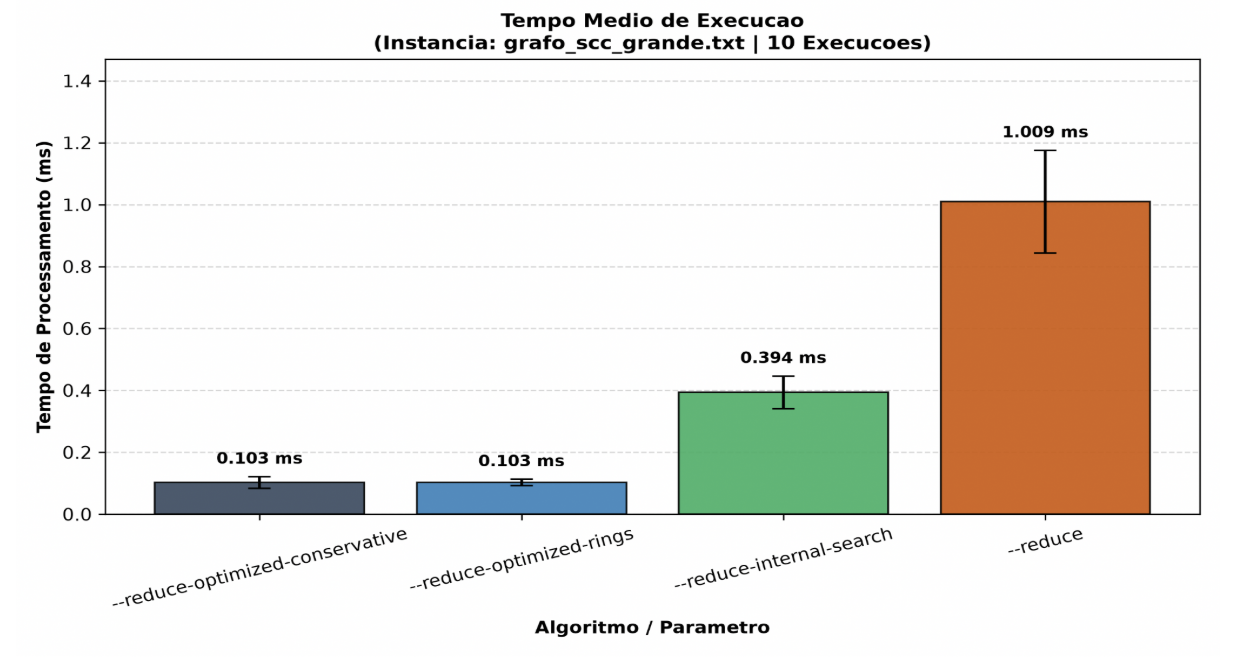
\includegraphics[width=0.45\textwidth]{img/grafico-1-tempo-medio-execucao.png}
    \caption{Tempo médio de execução dos algoritmos na instância geral.}
    \label{fig:tempo-medio-execucao}
\end{figure}

O Gráfico~\ref{fig:tempo-medio-execucao} evidencia a diferença de custo entre as estratégias. O \textit{baseline} \texttt{--reduce} apresentou o pior desempenho, com tempo médio de 1{,}009 ms, resultado esperado por testar a redundância das arestas de forma direta e repetitiva. A variante \texttt{--reduce-internal-search} reduziu esse custo para 0{,}394 ms ao restringir as buscas ao interior das componentes fortemente conexas, mantendo a mesma lógica de preservação de atingibilidade. Já as abordagens \texttt{--reduce-optimized-conservative} e \texttt{--reduce-optimized-rings} ficaram no menor patamar de tempo, ambas próximas de 0{,}103 ms, pois evitam buscas internas sucessivas em larga escala.

\begin{figure}[H]
    \centering
    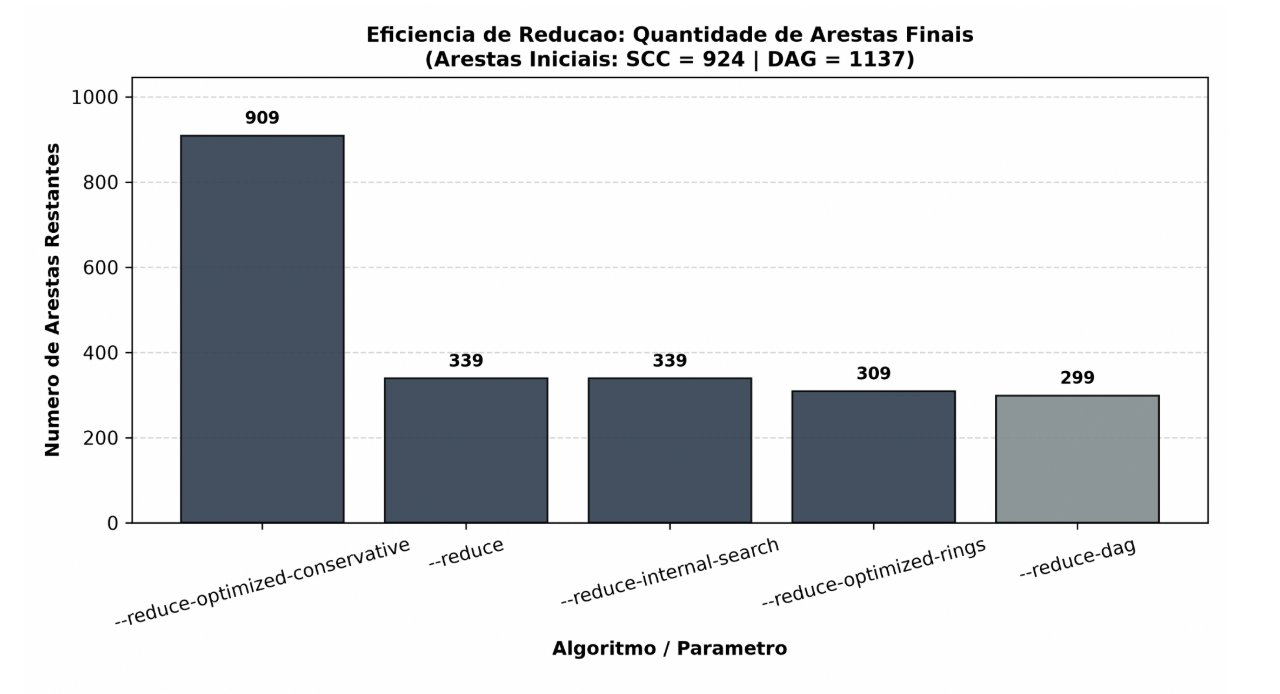
\includegraphics[width=0.43\textwidth]{img/grafico-2-eficiencia-reducao.png}
    \caption{Eficiência de redução: quantidade de arestas finais após a compressão.}
    \label{fig:eficiencia-reducao}
\end{figure}

O Gráfico~\ref{fig:eficiencia-reducao} mostra que velocidade isolada não implica boa redução. A abordagem conservadora manteve 909 das 924 arestas originais, removendo apenas uma fração pequena do grafo. Embora seja rápida, sua compressão é limitada por preservar integralmente o interior das SCCs. Em contraste, o \textit{baseline} \texttt{--reduce} e a variante \texttt{--reduce-internal-search} reduziram o grafo para 339 arestas finais, preservando a condição de subgrafo estrito. Assim, na instância com SCCs, a busca interna alcançou a mesma redução do baseline com custo substancialmente menor.

A variante \texttt{--reduce-optimized-rings} obteve 309 arestas finais em análise demonstrativa, delimitando o patamar máximo de compressão quando $E' \subseteq E$ é relaxado. Por poder introduzir arestas sintéticas, não garante $E' \subseteq E$ em todos os casos e não deve ser interpretada como redução transitiva estrita, sendo seus resultados incomparáveis às variantes válidas. A variante \texttt{--reduce-dag}, por sua vez, obteve 299 arestas finais sobre uma instância acíclica distinta, servindo apenas como referência de escopo.

\begin{figure}[H]
    \centering
    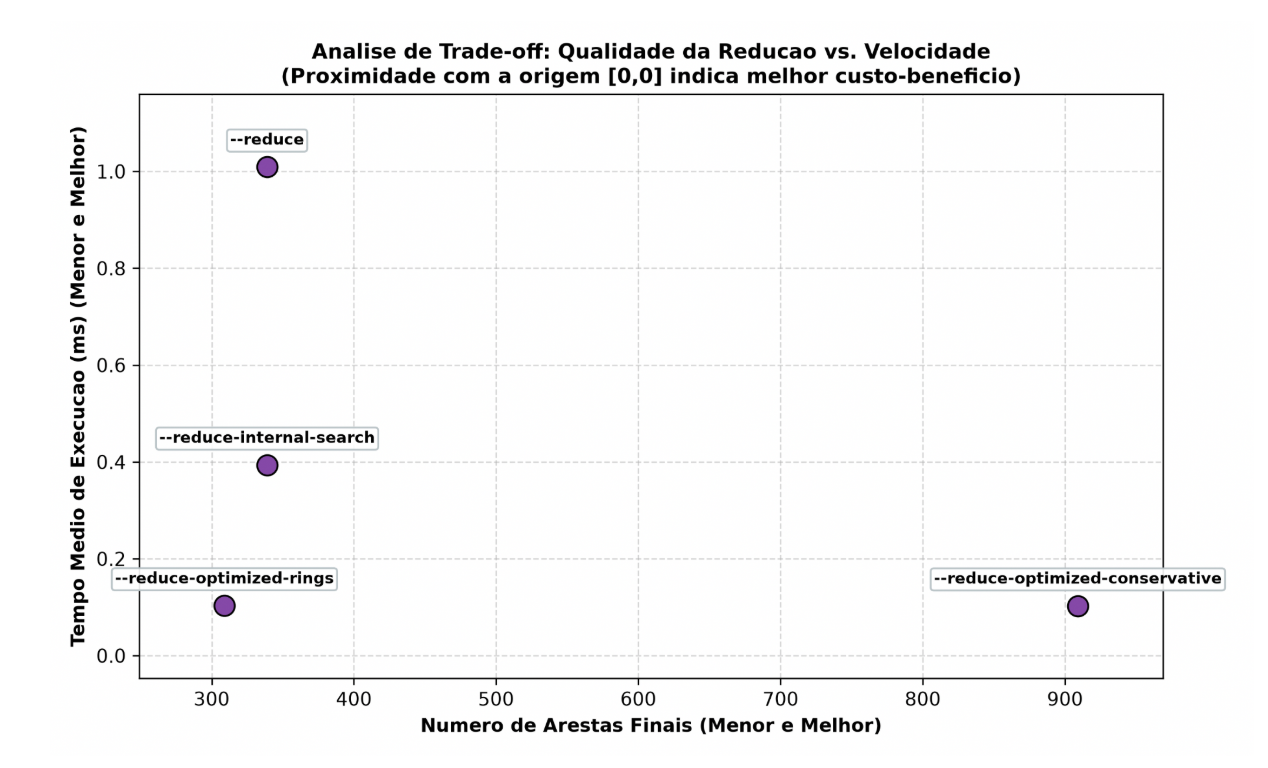
\includegraphics[width=0.41\textwidth]{img/grafico-3-tradeoff-qualidade-velocidade.png}
    \caption{Análise de \textit{trade-off}: qualidade da redução versus velocidade.}
    \label{fig:tradeoff-qualidade-velocidade}
\end{figure}

O Gráfico~\ref{fig:tradeoff-qualidade-velocidade} sintetiza o compromisso entre velocidade e qualidade da redução. O \texttt{--reduce} serve como referência de corretude ao maior custo computacional; a variante conservadora é rápida, porém pouco agressiva. O \texttt{--reduce-internal-search} apresenta o melhor resultado entre as soluções válidas: preserva a atingibilidade, mantém $E' \subseteq E$ e reproduz a mesma quantidade de arestas finais do \textit{baseline} com tempo significativamente menor.

Em todas as variantes válidas, a comparação de atingibilidade indicou 0 divergências, confirmando que as remoções não alteraram os conjuntos de vértices alcançáveis. Esse resultado reforça que a redução só é satisfatória quando combina compressão, desempenho e preservação integral da alcançabilidade.

\section{Conclusão}

Neste trabalho, apresentamos abordagens algorítmicas para a redução transitiva em grafos direcionados, combinando condensação de componentes cíclicos e heurísticas locais. Os resultados experimentais demonstram que a redução por restrição de escopo por componente e a Heurística de Busca Interna, relacionada ao problema MEG (\textit{Minimum Equivalent Graph}), superam a força bruta em eficiência computacional, alcançando elevada compressão sem comprometer a atingibilidade sistêmica. A variante \texttt{--reduce-internal-search} obteve a mesma quantidade de arestas finais do \textit{baseline} na instância com SCCs, porém com menor tempo médio de execução, preservando a condição $E' \subseteq E$.

O método proposto reduz significativamente a dimensionalidade das arestas, com validação empírica indicando 0 divergências de atingibilidade nas variantes avaliadas. Ainda assim, em grafos direcionados gerais com ciclos, a busca interna deve ser interpretada como heurística prática de redução, e não como garantia de minimização global. Uma limitação teórica reside no \textit{trade-off} necessário para manter a otimização em tempo polinomial, restringindo o escopo a estruturas direcionadas. A abordagem de anéis, embora apresente maior compressão, deve ser entendida apenas como contraponto experimental, pois pode introduzir arestas sintéticas, violando a premissa de subgrafo estrito, na qual $E'$ deve ser subconjunto de $E$.

Conforme discutido, a transposição desses métodos para grafos não direcionados exige uma adaptação conceitual. Nesse cenário, preservar atingibilidade equivale a preservar conectividade entre vértices de uma mesma componente conexa, de modo que o problema se aproxima da construção de uma floresta geradora, ou de uma árvore geradora mínima quando houver pesos associados. Assim, o caso não direcionado não corresponde diretamente à mesma semântica da redução transitiva em grafos direcionados.

Finalmente, este trabalho contribui para rotinas de simplificação estrutural em Ciência da Computação, com aplicações em otimização de rotas e gerenciamento de dependências de software. Pesquisas futuras podem explorar a implementação dessas heurísticas em grafos dinâmicos e bancos de dados de larga escala, consolidando a abordagem de condensação com restrição por componente como caminho promissor para otimização de redes.

\bibliographystyle{apalike-sol}
\bibliography{refs}

\end{document}